\section{Variational Autoencoders}
\label{sec:vae}
Variational autoencoders (VAE) have been developed concurrently in 2014 by Kingma et al.\cite{vae:2014} and Rezende et al.\cite{dlgm:2014}.
%The proposed framework resembles the encoder-decoder architecture, using a probabilistic encoder and decoder.
The general idea of VAEs is to have an encoder-decoder architecture where input $x$ gets mapped to a specific distribution defined in the latent space $z$ from which we sample in order to reconstruct the input.


%\begin{figure}[htb]
%\centering
%\resizebox{5cm}{!}{\definecolor{cdfdfdf}{RGB}{223,223,223}
\definecolor{cffffff}{RGB}{255,255,255}


\begin{tikzpicture}[y=0.80pt, x=0.80pt, yscale=-1.000000, xscale=1.000000, inner sep=0pt, outer sep=0pt]
\begin{scope}[cm={{1.25,0.0,0.0,-1.25,(0.0,1052.3622)}}]
  \begin{scope}[shift={(306.491,697.587)}]
    \path[draw=black,fill=cdfdfdf,line join=miter,line cap=butt,miter
      limit=10.00,nonzero rule,line width=0.319pt] (9.9628,0.0000) .. controls
      (9.9628,5.5023) and (5.5023,9.9628) .. (0.0000,9.9628) .. controls
      (-5.5023,9.9628) and (-9.9628,5.5023) .. (-9.9628,0.0000) .. controls
      (-9.9628,-5.5023) and (-5.5024,-9.9628) .. (0.0000,-9.9628) .. controls
      (5.5023,-9.9628) and (9.9628,-5.5024) .. (9.9628,0.0000) -- cycle;
  \end{scope}
    \path[cm={{1.0,0.0,0.0,-1.0,(303.468,695.373)}},fill=black,nonzero rule]
      (0.0000,0.0000) node[above right] (text4171) {$x$};
  \begin{scope}[shift={(306.491,697.587)}]
    \path[draw=black,fill=cffffff,line join=miter,line cap=butt,miter
      limit=10.00,nonzero rule,line width=0.319pt] (9.9628,48.6708) .. controls
      (9.9628,54.1732) and (5.5024,58.6336) .. (0.0000,58.6336) .. controls
      (-5.5023,58.6336) and (-9.9628,54.1732) .. (-9.9628,48.6708) .. controls
      (-9.9628,43.1685) and (-5.5024,38.7081) .. (0.0000,38.7081) .. controls
      (5.5023,38.7081) and (9.9628,43.1685) .. (9.9628,48.6708) -- cycle;
  \end{scope}
    \path[cm={{1.0,0.0,0.0,-1.0,(303.945,744.043)}},fill=black,nonzero rule]
      (0.0000,0.0000) node[above right] (text4181) {$z$};
    \path[cm={{1.0,0.0,0.0,-1.0,(260.848,741.767)}},fill=black,nonzero rule]
      (0.0000,0.0000) node[above right] (text4187) {$\phi$};
    \path[cm={{1.0,0.0,0.0,-1.0,(345.199,742.798)}},fill=black,nonzero rule]
      (0.0000,0.0000) node[above right] (text4193) {$\theta$};
  \begin{scope}[shift={(306.491,697.587)}]
    \path[draw=black,dash pattern=on 2.39pt off 2.39pt,line join=miter,line
      cap=butt,miter limit=10.00,line width=0.319pt] (-38.5088,48.6708) --
      (-10.9710,48.6708);
  \end{scope}
  \begin{scope}[shift={(295.52,746.258)}]
    \path[draw=black,fill=black,line join=miter,line cap=butt,miter
      limit=10.00,nonzero rule,line width=0.319pt] (-5.2035,2.3356) --
      (0.2989,0.0000) -- (-5.2035,-2.3356) -- (-5.2035,2.3356) -- cycle;
  \end{scope}
  \begin{scope}[shift={(306.491,697.587)}]
    \path[draw=black,line join=miter,line cap=butt,miter limit=10.00,line
      width=0.319pt] (38.5088,48.6708) -- (10.9710,48.6708);
  \end{scope}
  \begin{scope}[cm={{-1.0,0.0,0.0,-1.0,(317.462,746.258)}}]
    \path[draw=black,fill=black,line join=miter,line cap=butt,miter
      limit=10.00,nonzero rule,line width=0.319pt] (-5.2035,2.3356) --
      (0.2989,0.0000) -- (-5.2035,-2.3356) -- (-5.2035,2.3356) -- cycle;
  \end{scope}
  \begin{scope}[shift={(306.491,697.587)}]
    \path[draw=black,line join=miter,line cap=butt,miter limit=10.00,line
      width=0.319pt] (38.5088,45.5084) -- (7.1087,8.4005);
  \end{scope}
  \begin{scope}[cm={{-0.64792,-0.7657,0.7657,-0.64792,(313.6,705.988)}}]
    \path[draw=black,fill=black,line join=miter,line cap=butt,miter
      limit=10.00,nonzero rule,line width=0.319pt] (-5.2035,2.3356) --
      (0.2989,0.0000) -- (-5.2035,-2.3356) -- (-5.2035,2.3356) -- cycle;
  \end{scope}
  \begin{scope}[shift={(306.491,697.587)}]
    \path[draw=black,dash pattern=on 2.39pt off 2.39pt,line join=miter,line
      cap=butt,miter limit=10.00,line width=0.319pt] (-7.1856,7.1856) .. controls
      (-16.6444,16.6438) and (-16.6444,32.0271) .. (-7.7582,40.9132);
  \end{scope}
  \begin{scope}[cm={{0.7071,0.7071,-0.7071,0.7071,(298.733,738.5)}}]
    \path[draw=black,fill=black,line join=miter,line cap=butt,miter
      limit=10.00,nonzero rule,line width=0.319pt] (-5.2035,2.3356) --
      (0.2989,0.0000) -- (-5.2035,-2.3356) -- (-5.2035,2.3356) -- cycle;
  \end{scope}
  \begin{scope}[shift={(306.491,697.587)}]
    \path[draw=black,line join=miter,line cap=butt,miter limit=10.00,line
      width=0.319pt] (0.0000,38.5088) -- (0.0000,10.9710);
  \end{scope}
  \begin{scope}[cm={{0.0,-1.0,1.0,0.0,(306.491,708.558)}}]
    \path[draw=black,fill=black,line join=miter,line cap=butt,miter
      limit=10.00,nonzero rule,line width=0.319pt] (-5.2035,2.3356) --
      (0.2989,0.0000) -- (-5.2035,-2.3356) -- (-5.2035,2.3356) -- cycle;
  \end{scope}
    \path[cm={{1.0,0.0,0.0,-1.0,(308.318,675.918)}},fill=black,nonzero rule]
      (0.0000,0.0000) node[above right] (text4239) {N};
  \begin{scope}[shift={(306.491,697.587)}]
    \path[draw=black,line join=miter,line cap=butt,miter limit=10.00,line
      width=0.319pt] (16.5376,62.3527) -- (-16.5376,62.3527) .. controls
      (-18.7386,62.3527) and (-20.5228,60.5685) .. (-20.5228,58.3676) --
      (-20.5228,-21.2037) .. controls (-20.5228,-23.4046) and (-18.7386,-25.1888) ..
      (-16.5376,-25.1888) -- (16.5376,-25.1888) .. controls (18.7386,-25.1888) and
      (20.5228,-23.4046) .. (20.5228,-21.2037) -- (20.5228,58.3676) .. controls
      (20.5228,60.5685) and (18.7386,62.3527) .. (16.5376,62.3527) -- cycle;
  \end{scope}
\end{scope}

\end{tikzpicture}

}
  %\caption{Graphical model of the variational autoencoder \cite{vae:2014}}
  %\label{fig:vae_architecture}
%\end{figure}


%However, in addition to this autoencoder structure an additional regularizer forces the latent space to have a specific simple form.
%To achieve this, variational-based methods are used to output a distribution on the latent space instead of directly emitting samples.

The probabilistic encoder generally implemented as feed-forward network receives input from the dataset and outputs parameters of a distribution. For example the parameters for a gaussian distribution with diagonal covariance, in which case the network emits the mean $\mu$ and $\sigma$ used to define the gaussian distribution $\mathcal{N}(\mu,\sigma \times I)$, where $I$ is the identity matrix.\\

Using gradient-based optimization techniques enables the encoder network to be trained to output distributions similar to the true posterior $p(z|x)$.
In addition to this inference network there is a generator network which transforms points $z$ in the latent space back to the data space while trying to minimize the reconstruction error.


One useful aspect of this approach is the possibility to train both networks using error backpropagation due to the use of neural networks as function approximators.\\\\

Such function approximator will emit the variational parameters $\phi$ of the probability encoder distribution $q_\phi(z|x)$.
Equally for the probabilistic decoder which constructs a distribution $p_\theta(x|z)$ with the parameters $\theta$.
This architecture is shown in Figure \ref{fig:vae_architecture} with a one-dimensonal gaussian prior.
\\


\begin{figure}[h]
  \centering
  \includestandalone[width=\linewidth,mode=buildnew]{media/vae_conceptual}
  \caption[VAE architecture]{simplified VAE architecture using a gaussian prior on $z$}
  \label{fig:vae_architecture}
\end{figure}

The key insight on how the variational autoencoder is able to optimize $q_\phi(z|x)$ to approach the true data posterior distribution $p(z|x)$ is in defining a variational lower bound which is used to push the approximated $q_\phi(z|x)$ towards $p(z|x)$. We will discuss this lower bound $\mathcal{L}$ and its derivation in detail in the following sections.

\newpage

%The approach taken by VAE is instead of sampling directly to a latent space $z$ it uses a inference network to output parameters of an distribution on $z$. 

%One of the useful aspects using this approach is that the inference problem of computing $p(z|x)$ is posed as optimizing the inference network to output good values for distributions approximating $p(z|x)$.
%The model maps the input $x$ using an inference network to a distribution $q_\theta(z|x)$ while a generative network maps samples from the latent space $z$ to to the data space $~x \

%Using an inference network allows the model to be trained fully using gradient-based methods and error backpropagation.\\
%The relation to other autoencoders becomes appearant when the inference networks gets renamed to \emph{probabilistic encoder} $q_\theta(z|x)$ and the generator to \emph{probabilistic decoder} $p_\phi(x|z)$ whereas the encoder maps samples $x$ from the data space to latent space $z$, or more precisely parameters of the distribution $q_\theta(z|x)$.
%Meanwhile does the decoder maps variables from the latent space $z$ back into the data space as shown in figure \ref{fig:vae_architecture}.\\





%VAEs couple a generator network with an inference network in which efficient inference and learning can be performed, thus allowing the model to be trained purely using gradient-based methods.

%which uses variational inference to perform efficient inference and learning in deep latent models.
%Deep latent models are based on the assumption that input data can be explained using non-linear transformations coming from simple distributions. \cite{rezende:2014} (check!?).

%\paragraph{Inference problem}
%The problem variational-based methods can solve is approximating intractable posterior distributions.\\

%Given a dataset $X = { x^{(1)}, x^{(2)}, \dots, x^{(n)}}$ and a model with observations $x \in X$ and hidden variables $z$. The inference problem is posed as computing the posterior distribution $p(z|x)$ 
%\begin{equation}
  %\label{eq:intractable_posterior}
  %p(z|x) = \frac{p(x|z) p(z)}{p(x)}
%\end{equation}
%However, computing the right-hand side of equation \ref{eq:intractable_posterior} is intractable due to the exponentially many configurations of the hidden variables. As such it is often needed to use approximate inference such as variational inference.

\subsection{Approximated Inference}
A problem which often arises in directed generative models is the \emph{inference problem}.
As discussed in the introduction~\ref{sec:introduction}, we assume that the observations are stochastically dependent on some latent variables.
Inference is called the process of coming up with values of $z$ which can produce the observations, which formally means evaluating $p(z|x)$ where $z$ are the latent variables and $x$ observations.
\begin{equation}
  p(z|x) = \frac{p(x|z)p(z)}{p(x)}\\
  \label{eq:intractable_posterior}
\end{equation}
where
\begin{conditions}
  p(z|x) & posterior distribution\\
  p(x|z) & likelihood of $x$ given $z$\\
  p(z)   & prior distribution of $z$\\
\end{conditions}
Using Bayes's rule we can expand the posterior distribution $p(z|x)$ as shown in Equation~\ref{eq:intractable_posterior}.
Note that to evaluate the denominator $p(x)$, all hidden variables need to be marginalized: $p(x) = \int p(x,z) dz$.\\
Due to the possibly large number of hidden variables, this integral can be high-dimensional and therefore difficult to calculate.
This integral can be difficult to compute and needs to be approximated.
However, for a large number of hidden variables, this integral is intractable to compute exactly and therefore needs to be approximated~\cite[p.~461-462]{bishop:2006}.
In order to approximate those intractable posterior distributions, we discuss two commonly used techniques:  Markov chain Monte Carlo and variational inference.

\paragraph{Markov chain Monte Carlo}
MCMC methods are a class of techniques which can be used to sample from a large class of distribution where direct sampling is not applicable~\cite[Chapter~11.2]{bishop:2006}.
For the variational autoencoder, where we want to approximate the posterior distribution $p(z|x)$ a method called \emph{Gibbs sampling}~\cite[Chapter~11.3]{bishop:2006} can be used to obtain samples from that conditional distribution by constructing a Markov chain with the desired equilibrium distribution.
%
One advantage of MCMC methods is that the resulting distribution is proven to be exactly the desired distribution~\cite[Chapter~11.3]{bishop:2006}.
However, due to the problems of mixing between mixing modes~\cite[Chapter~17.5]{deeplearning:2016} and slow convergence rate\cite[p.~603]{deeplearning:2016} these methods are impractical for usage in the inner loop of optimization techniques.

\paragraph{Variational Inference}
% variational inference
Due to the possibly slow convergence of MCMC methods, variational inference (VI)~\cite[Chapter~19.4]{deeplearning:2016} is used in the variational autoencoder.
VI works by picking a specific distribution restricted to a family of distributions which matches the posterior most closely. This means that VI is used to turn the inference problem into an optimization technique, allowing for gradient-based optimization.
%TODO: more on advantages and disadvantages
Using VI yields better performance at the sacrifice of theoretical guarantee of matching the posterior distribution.


More specifically, VI turns the inference problem of computing $p(z|x)$ where $z$ are the hidden and $x$ the observed variables into an optimization problem, where we can use gradient-based methods.


\subsubsection{Kullback-Leibler Divergence}
In order to approximate one distribution $Q$ to another distribution $P$, there needs to be a measurement of how close $Q$ is to $P$.
One commonly used measurement is called Kullback-Leibler (KL) divergence\cite{kl_div:1951} which enables the variational inference methods to choose appropiate distributions.
%\paragraph{The Kullback-Leibler Divergence} (KL divergence) is a measurement for the difference between two probability distributions. $\mathcal{D}_{\mathrm{KL}}(P \| Q)$ can informally described as the amount of information which is lost when using $Q$ to represent $P$.
The KL divergence from $Q$ to $P$ is defined in Equation \ref{eq:kl_div}.
\begin{equation}
  \label{eq:kl_div}
  \mathcal{D}_{\mathrm{KL}}(P || Q) = \mathbb{E}_{x \sim P(x)}\bigg[log \frac{P(x)}{Q(x)}\bigg]
\end{equation}
\todo[inline]{Add some description to the equation above, logarithmic difference between P and Q, bla bla expectation}
%For discrete probability distributions $P$ and $Q$, the KL divergence from $Q$ to $P$ is defined\cite{kl_div:1951} in equation \ref{eq:kl_div_disc}:
%\begin{equation}
  %\label{eq:kl_div_disc}
  %\mathcal{D}_{\mathrm{KL}}(P || Q) = \sum_{i} P(i) \log \frac{P(i)}{Q(i)}
%\end{equation}
%For continuous distributions $P$ and $Q$ the KL divergence is defined similarly in equation \ref{eq:kl_div_cont}.
%\begin{equation}
  %\label{eq:kl_div_cont}
  %\mathcal{D}_{\mathrm{KL}}(P || Q) = \int P(i) \log \frac{P(i)}{Q(i)} di
%\end{equation}

Note that divergence does not obey the triangle inequality and is also not symmetrical, therefore it does not qualify as a metric.
$\mathcal{D}_{\mathrm{KL}}(P||Q)$ can nevertheless be understood as a measure of the difference between $P$ and $Q$ and is as such used in the variational inference.


\newpage


%The need for such optimizations techniques


%is suited to approximate intractable posterior distributions over a set of hidden variables given observations.
%Variational-based methods have become a popular choice for inference problems, 
%Variational Inference (VI) is a method for approximating intractable posterior distributions over a set of hidden varibales given observations.

%The term \emph{variational} derives from the calculus of variations, which is a field in mathematical analysis dealing with choosing the best function $q$ from a set of functions $Q$. In the case of variational inference, this $Q$ denotes a class of distributions and the variational parameters are the parameters which are used to define $q \in Q$.
%VI is a alternative to markov chain monte carlo (MCMC) methods like gibbs sampling, due to lower computational cost.
%However, there is no guarantee that VI methods will asymptotically reach the optimimum in contrast to MCMC.

%Given this assumption, building a good representation in the latent space is crucial for minimal reconstruction error as well as good generative modelling in practice(?).

% TODO: add clarification that q/p are deep nets!

%\newpage

%Performing statistical inference means computing $p(z|x)$ which is intractable in all but very simple cases (integrating over it, show calc).

%In this setup we have observed variables $x$ from which we would like to infer latent variables $z$


%Variational Autoencoders (VAE) have been a popular choice for unsupervised learning of complicated distributions (citation needed) and generative modelling.
%In order to generate data from unknown and mostly intractable distributions, we need approximations.
%There are basically two approaches for sampling from these distributions,
%first there are approximate samples (MCMC, gibbs sampling, etc) which try to directly approximate $p(x)$.
%Variational Autoencoders instead try to match an easier to compute distribution $q(x)$ to $p(x)$.
%By using this approach, VAEs are computationally less intensive (citation?) but have the drawback of being more restricted in their modelling approach.
%Practically, this means that with more computation MCMC methods approach $p(x)$, while there is no such guarantee for variational methods (--> not for all).

%VAE can be learned with just backpropagation (paper,TODO), but they differ from denoising and sparse autoencoders due to the different loss function.


%VAEs are built on top of neural networks and are designed in a way to allow training with gradient-based methods.
%Learning and inference are reasonable efficient and relatively easy to implement and show decent results, but have been overshadowed by more recent adversarial approaches (citation needed!!,see \ref{sec:gan}).

%\subsection{Architecture}
%\label{sub:vae_architecture}

%$p(x,z)$ is the joint probability distribution over both input and latent variables while $p(z|x)$ is the conditional probability of the latent variables given input data.
%Inferring the posterior distribution $p(z|x)$ is particularly interesting, because it means to enable learning parameters for good latent space representation.
%$p(z|x)$ can be expanded using bayes rule to $\frac{p(x|z) p(z)}{p(x)}$.
%Computing the nominator is straightforward, $p(z)$ is the probability distribution we chose for the latent space, oftenmost simply a gaussian.
%$p(x|z)$ is easy to compute as well, ...? (forward pass?).\\
%Meanwhile is the denominator difficult to evaluate, because it requires to consider all possible input combinations.
%What we do instead in the variational autoencoders is to derive a lower-bound on $p(z|x)$ using a auxiliary distribution called $q_\theta(z|x)$. The subscript $\theta$ indicates that the distribution is parametrized by an variational term, so that for one $\theta$, $q_\theta(z|x) \approxeq p(z|x)$ holds ($q(z|x)$ doesn't need to depend on $x$).

%VAE just like other autoencoders encode the input data into a latent space similar to compression of data and is able to decode a vector of latent variables into output while trying to match the output to the input.
%But in contrast to other autoencoders (sparse, denoising), we enforce a specific distribution on the latent space.
%This allows to sample from this distribution and generate output which will look similar to the data on which the VAE has been trained.
%\ref{fig:vae_architecture}.

%\paragraph{Relation to Auto-Encoders}
%The variational autoencoder has the same encoding-decoding architecture as other autoencoders, for example sparse or denoising autoencoders.
%But in contrast to these autoencoders, the VAE enforces a probability distribution on the learned latent space $z$.
%In particular, the framework encourages the model to learn a representation that is close to $p(z)$ (which usually is an isotropic multivariate gaussian distribution) by including the KL divergence in the objective function.
%Similar to other autoencoder frameworks VAE provides an encoder as well as a decoder model, but in contrast to other autoencoders both networks are probabilistic. This means that the model described by the VAE framework can be seen as a jointly trained probabilistic encoder and probabilistic decoder.
%One of the main differences is that the VAE framework enforces a specific prior distribution on the latent space, most of the time simply an isotropic gaussian.



\subsection{Objective Function}
%The objective function of the VAE consists of the reconstruction error and the regularizer.
%$\mathcal{L}$ learns both the encoder as well as the decoder with their respective parameters $\phi$ and $\theta$.
% probabilistic encoder $q_\phi(z|x)$ (produces z values from which x could've been generated)
% probabilistic decoder $p_\theta(x|z)$
%We will discuss both terms in detail below following the derivation of the lower variational bound $\mathcal{L}$ and the rewritten objective function.
Following the thoughts earlier, we wish to derivate an objective function which can be used to perform gradient-based optimization in the model.\\
We construct the approximate posterior $q_\phi(z|x)$ which we want to approach the true data posterior $p(z|x)$.
When using the KL divergence as measurement for difference between two distributions the goal for which we want to optimize becomes the following.
\begin{equation}
  \label{eq:vae_obj}
  q_\phi^{*}(z|x) = \arg\min_{\phi} \mathcal{D}_{\mathrm{KL}} \big(q_\phi(z|x) || p(z|x)\big)
\end{equation}

However we are not able to optimize Equation \ref{eq:vae_obj} directly, as the intractable evidence $p(x)$ appears during the expansion of the posterior $p(z|x)$ to $\frac{p(x|z)p(z)}{p(x)}$.\\
The denominator $p(x)$ can be computed by marginalizing out the hidden variables $z$: 
\begin{equation}
  \label{eq:integral}
p(x) = \int p(x,z) p(z) dz
\end{equation}

Computing the integral in Equation \ref{eq:integral} requires the evaluation of every possible configuration over the hidden variables $z$ and is therefore intractable.\\\\

Instead of directly optimizing for the true posterior, we construct an evidence lower bound (ELBO) $\mathcal{L}$ which we can maximize which is equivalent to minimizing the KL divergence between $q_\phi(z|x)$ and $p(z|x)$ without explicity evaluating the evidence.\\



\paragraph{Derivation of the evidence lower bound}
Based on \cite[p.~698]{deeplearning:2016}.
\begin{align*}
  \log p(x)\\
  &= \int_z q_\phi(z|x) \log p(x) dz\\
  &= \int_z q_\phi(z|x) \log \frac{p_\theta(x,z)}{p_\theta(z|x)} dz \tag{Bayes' rule}\\
  &= \int_z q_\phi(z|x) \log\bigg(\frac{p_\theta(z,x)}{q_\phi(z|x)} \frac{q_\phi(z|x)}{p_\theta(z|x)}\bigg) dz \tag{Chain rule}\\
  &= \int_z q_\phi(z|x) \bigg(\log\frac{p_\theta(z,x)}{q_\phi(z|x)} + \log\frac{q_\phi(z|x)}{p_\theta(z|x)}\bigg) dz\\
  &= \int_z q_\phi(z|x) \log \frac{p_\theta(z,x)}{q_\phi(z|x)} dz + \int_z q_\phi(z|x) \log\frac{q_\phi(z|x)}{p_\theta(z|x)} dz\\
  &= \underbrace{\int_z q_\phi(z|x) \log \frac{p_\theta(z,x)}{q_\phi(z|x)} dz}_{= \mathcal{L}}+ \underbrace{\mathcal{D}_{\mathrm{KL}}\big(q_\phi(z|x) \| p_\theta(z|x)\big) dz}_{\geq 0}\\
  &\geq \mathcal{L}\\
\end{align*}

$\mathcal{L}$ is called the evidence lower bound with respect to $\log p(x)$.
We further rewrite $\mathcal{L}$ in order decompose the term into two separate terms, the reconstruction error $\mathcal{L}_{rec}$ and the regularizer $\mathcal{L}_{reg}$.

\begin{align*}
  \mathcal{L}
  &= \int q_\phi(z|x) \log\frac{p_\theta(z,x)}{q_\phi(z|x)} dz\\
  &= \int q_\phi(z|x) \log\frac{p(z) p_\theta(x|z)}{q_\phi(z|x)} \tag{we assume that x is conditionally dependent on z} dz\\
  &= \int q_\phi(z|x) \bigg(\log\frac{p(z)}{q_\phi(z|x)} + \log p_\theta(x|z)\bigg) dz\\
  &= -\int q_\phi(z|x) \log\frac{q_\phi(z|x)}{p(z)} dz + \int q_\phi(z|x) \log p_\theta(x|z) dz\\
  &= -\mathcal{D}_{\mathrm{KL}}\big(q_\phi(z|x) \| p(z)\big) + \int q_\phi(z|x) \log p_\theta(x|z) dz\\
  &= \underbrace{-\mathcal{D}_{\mathrm{KL}}\big(q_\phi(z|x) \| p(z)\big)}_{\mathcal{L}_{reg}} + \underbrace{\mathbb{E}_{z \sim q_\phi(z|x)}\big[ \log p_\theta(x|z)\big]}_{\mathcal{L}_{rec}}\\
  &= \mathcal{L}_{reg} + \mathcal{L}_{rec}
\end{align*}



\paragraph{Regularization term $\mathcal{L}_{reg}$} encourages the model to learn simple representations in latent space, due to the negative KL divergence between the learned variational distribution $q_\phi(z|x)$ and the latent space prior distribution $p(z)$.

%The regularizer is also important to the VAE as it ensures that the model learns generalized representations in latent space.

Using the example of handwritten digits it appears why this regularizer term $\mathcal{L}_{reg}$ is important for the model to learn generalized representations in latent space.
Suppose we have two data points from the dataset which both represent the same handwritten digit.
Ideally, our model would learn representations in latent space to be fairly close to ensure the model has learned to generalize the semantics. Without $\mathcal{L}_{reg}$ the model would assign each data example a different representation in latent space with a distribution collapsing to that single point. This behaviour is undesired and is as such penalitized.

%Suppose two data points with similar input
%Without $\mathcal{L}_{reg}$ the encoder would encode data points we want to have similar representations, fo

%The regularizer term is also important to prevent the model from collapsing into a single point.

\vspace{2cm}

\paragraph{Reconstruction error $\mathcal{L}_{rec}$} measures how well the decoder reconstructs the input data using the latent space $z$.
This error is measured using the negative log-likelihood of the conditional probability distribution $p_\theta(x|z)$ where $z$ is sampled from $q_\phi(z | x)$.\\
$\mathcal{L}_{\mathrm{rec}}$ is necessary to force the encoder to produce latent variables which can be used to reconstruct the input data well.

\newpage

%\begin{figure}[htb]
%\centering
%\includestandalone[width=\linewidth,mode=buildnew]{media/vae_multiple_layers}
  %\caption{VAE with multiple stochastic layers }\label{fig:vae_multiple_layers}
  %\medskip
  %\small
  %The left upward arrows indicate the recognition networks $q(h_1|x)$ and $q(h_2|h_1)$.
  %Note that the recognition networks can have multiple deterministic layers (including non-linearities).\\

  %$p(h_2)$ denotes the probability distribution over the highest(?) latent space.\\

  %On the right, the two conditional distributions $p(h_1|h_2)$ and $p(x|h_2)$ are representing two networks used for the generative process.
%\end{figure}



\subsubsection{Reparameterization Trick}

\begin{figure}
  \centering
  \begin{tabular}{c:c}
    \subcaptionbox{without reparameterization}{\includestandalone[height=0.4\linewidth]{media/reparameterization_trick_without}}
      \quad \quad
    &
      \quad

    \subcaptionbox{with reparameterization applied}{\includestandalone[height=0.4\linewidth]{media/reparameterization_trick_with}}\\
  \end{tabular}
  \caption{Reparameterization Trick}
  \label{fig:rep_trick}
  \medskip
  \small
  Function $f_\theta(x)$ with inputs $x$ and (variational) parameters $\theta$ as computational graph.
  Left without and on the right with the reparameterization trick applied.\\
  Solid arrows show the forward pass and dashed arrows the error backpropagation using gradients.
  Rectangular nodes represent deterministic functions while circles indicate stochastic variables.
  %Note that backpropagation of gradients through stochastic nodes is problematic and adds bias (verify!)
\end{figure}

% more math:
% http://stats.stackexchange.com/questions/199605/how-does-the-reparameterization-trick-for-vaes-work-and-why-is-it-important
To be able to apply the backpropagation\cite{backprop:1988} algorithm to the loss function of the VAE without any injected noise it has to be both differentiable and deterministic.
However, as $z$ is sampled from the constructed probability distribution $q_\phi(z|x)$ it is stochastic.
This poses a problem, because the gradient can not be computed accurately due to the added noise.\\
In order to circumvent this restriction, the so-called ``reparameterization trick'' (as proposed by \cite{vae:2014} and \cite{dlgm:2014}) is applied.
Instead of drawing $z$ directly from $q_\phi(z|x)$, we first sample an auxiliary variable $\epsilon$ from the isotropic gaussian $\mathcal{N}(0, I)$. Then we apply Equation \ref{eq:rep_trick} to transform $\epsilon$ into $z$.
\begin{equation}
  \label{eq:rep_trick}
  z = \mu(x) + \Sigma^{1/2}(x)*\epsilon
\end{equation}
Note that this transformation is entirely deterministic and as such allows for backpropagation through the transformation into the variational parameters $\phi$.

Figure \ref{fig:rep_trick} expresses the reparameterization trick applied to an arbitrary function $f$ with the parameters $\theta$.\\
Using this trick, the whole VAE model can be trained using gradient-based optimization techniques.\\\\

Note further that in most common architectures, the distribution class enforced on the latent space is gaussian, there exists similar reparameterization techniques allowing different prior probability distributions on $z$.
%The core idea of VAEs is to match a distribution $q(x)$ to the desired $p(x)$ by enforcing a lower variational bound on $q(x)$ in a way that it seeks to match $p(x)$.
%In contrast to other autoencoders, VAEs behave differently due to this lower bound but they resemble the architecture of traditional autoencoders (sparse, denoising).




%We use VAEs when we have a complicated distribution $p_\theta(x,z)$ with unknown latent variables $z$.
%The prior distribution $p(z)$ over the latent structure is a centered isotropic(?) multivariate Gaussian denoted by $\mathcal{N}(z;0, I)$.
%The constructed architecture uses an probabilistic encoder $q_\theta(z|x)$ and a probabilistic decoder $p_\theta(x|z)$ in a form of neural networks, in the original paper MLP are used\cite{vae:2014} but there are various extensions (see \ref{sub:vae_extensions}, TODO).
%Because the posterior is intractable ($p_\theta(x)$), we instead approximately maximize the lower variational bound $L(\theta,\phi;x)$.\\
%\begin{equation}
  %\mathcal{L}(\theta,\phi;x) = -D_{KL}(q_\theta(z|x)||p(z)) + \mathbb{E}_{q_\theta(z|x)}[log_{p_\theta}(x|z)]
%\end{equation}




\newpage

\subsection{Learning}
\label{sub:vae_learning}
The probabilistic encoder $q_\phi(z|x)$ and decoder $p_\theta(x|z)$ are commonly implemented using deep neural networks.
To allow analytical computation of the ELBO, the prior on the latent space $z$ is often choosen to be the isotropic gaussian $p(z) = \mathcal{N}(0,1)$.

%To allow the computation of the KL divergence between $q_\theta(z|x)$ and the latent prior distribution $p(z)$ in closed form, the prior is an isotropic gaussian $\mathcal{N}(0, 1)$.


\begin{algorithm}
  \caption{Learning in the VAE model}
  \label{alg:vae}
  \begin{algorithmic}[1]
    %\Let{$\eta_d, \eta_g$}{Learning rate of discriminator and generator networks, respectively}
    %\Let{$\theta_d, \theta_g$}{Parameters of function approximators}
    \While{has not reached convergence}
      \Let{$x$}{sample from $p_{data}(x)$}
      \Let{$\epsilon$}{Random samples from noise prior $p(\epsilon)$}
      \Let{$g$}{Compute gradients $\nabla_{\theta,\phi}\mathcal{L}(\theta, \phi; x, \epsilon)$}
      \Let{$\theta, \phi$}{Update according to gradients $g$}
    \EndWhile
  \end{algorithmic}
\end{algorithm}

\subsection{Experiments}
In order to evaluate the inference performance and explore the learned latent space, the VAE has been implemented and trained\footnote{The source code is available on GitHub: \url{https://github.com/Spotlight0xff/deeplearning-seminar}}. Results of this experiments are shown in Figure \ref{fig:vae_experiments}.
%The model has been trained on the MNIST dataset \cite{mnist} with satisfactory generative performance as shown in figure \ref{fig:vae_experiments}



% define X correctly or replace formula below!
%$$
%q_\theta(z|x) = \mathcal{N}(z|\mu(X;\theta), \Sigma(X;\theta))
%$$

%Because we assume that $p(z)$ is also a multivariate Gaussian distribution, the KL-divergence can now be computed in closed form as follows\cite{derivations:2007}.
%\begin{align*}
  %\mathcal{D}_{\mathrm{KL}}\big[q_\theta(z|x) || p_\phi(z|x)\big] &= \mathcal{D}_{\mathrm{KL}}\big[\mathcal{N}(\mu_0,\Sigma_0) || \mathcal{N}(\mu_1,\Sigma_1)\big]\\
  %&= \frac{1}{2} \big(\mathrm{tr}\big(\Sigma_1^{-1}\Sigma_0\big) + \big(\big)\big)\\
%\end{align*}


%\subsection{Inference}
%\label{sub:vae_inference}
%In bayesian analysis, statistical inference is the process of evaluating $p(z|x)$ for a given conditional probability $p(x|z)$.
%% more info on marginal distribution, posterior inference etc!
%There are two approaches to performing this task, Markov chain Monte Carlo (MCMC) methods using Gibbs sampling and variational inference.
%MCMC methods have the advantage of being asympotically exact and unbiased while variational methods are computationally faster but biased and not guaranteed to approaching the distribution.
%In the case of VAE, variational inference is also used in order to backpropagate through the layers (using the reparameterization trick).


\begin{figure*}[t!]
    \centering
    \begin{subfigure}[t]{0.5\textwidth}
        \centering
        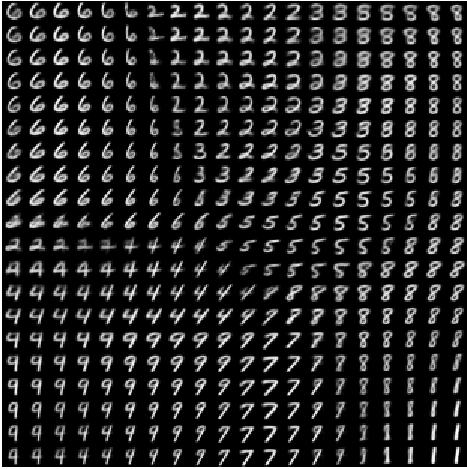
\includegraphics[height=7cm]{media/vae_manifold.pdf}
        \caption{Learned manifold using 2-dimensional latent space}
    \end{subfigure}%
    ~
    \begin{subfigure}[t]{0.5\textwidth}
        \centering
        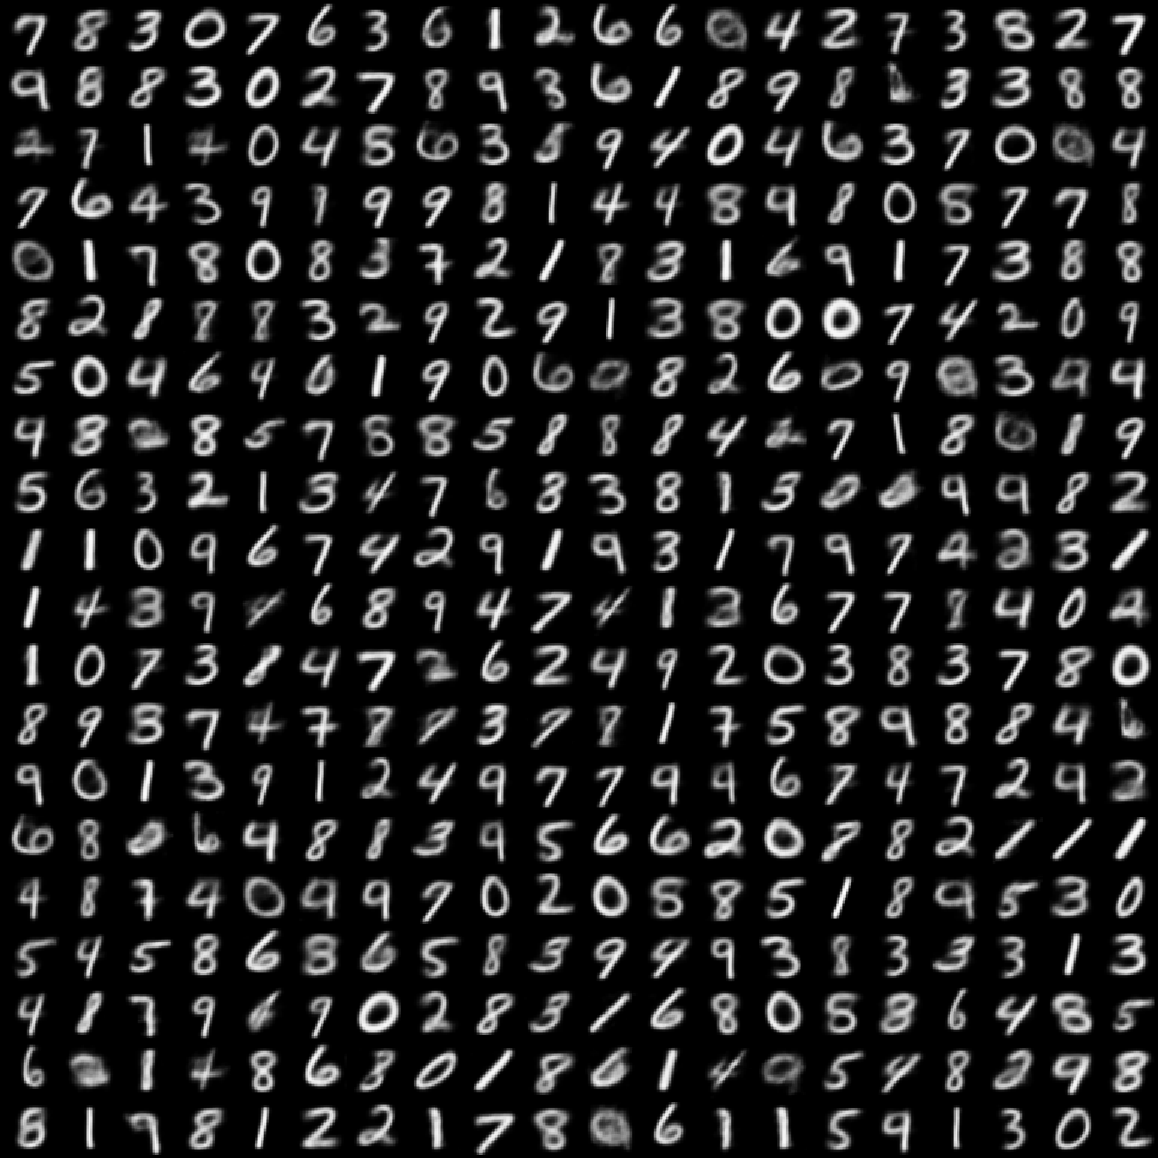
\includegraphics[height=7cm]{media/vae_samples.pdf}
        \caption{Generated images by sampling from latent space}
    \end{subfigure}
    \caption{Manifold Learning in the VAE}
    \label{fig:vae_experiments}
    \medskip
    \small
    (a) Evaluation of a variational autoencoder with 2 hidden layers with each 500 nodes and a two-dimensional latent space.
    The shown manifold has been plotted using samples uniformly samples in the range $[-3,-3]^2$ and then reconstructed using the decoder network $p_\theta(x|z)$. The results have shown that the model has learned to arrange the latent space in a sensible way by placing digits with high similarity near each other.\\
    (b) generative performance qualitively evaluated using samples in the data space by random sampling $z \sim p(z)$ and decoding $z$ using the decoder network. For this experiment an 50-dimensional latent space has been used.
\end{figure*}

%\subsection{Performance}
%\label{sub:vae_performance}

\newpage

\subsection{Extensions}
\label{sub:vae_extensions}

\subsubsection{Conditional VAE}
\label{ssub:cvae}
Instead of using VAEs in a completely unsupervised manner on a unlabeled dataset, it is also possible to learn from datasets where a small subset of datapoints has corresponding labels while most datapoints are still unlabeled.
Techniques learning from such datasets are called semi-supervised learning and can improve performance significantly.\\

To adjust the VAE model to the semi-supervised case, we have to add an random variable $y$ corresponding to the corresponding label if available.
Thus we can extend the distributions as shown below.

%The modified setup of the semi-supervised case for the variational autoencoder can be formalized as follows.
%Dataset $X$ of size $N$ with observations $x_i$ with $i<N$ where for some small subset of observations $x_i$ the corresponding labels $y_i$ are known.
%We denote the labelled subset as $~p_l(x,y)$ and the unlabelled dataset as $~p_u(x,y)$.
%\begin{equation}

%\end{equation}
%Instead of randomly generated data, generation of output conditioned on some prior information is needed.
%A few examples would be super-resolution of images (citation!), prediction of subsequent frames of an video or other prediction tasks

%Conditional VAE is a modification of the original VAE framework to support conditioning on another variable $y$ in addition to the input data $x$.

%To support conditional distributions, the following relations have to be rewritten:
\begin{itemize}
\item \textbf{Sampling from data space}: $x \sim p_\theta(x|y,z)$ instead of $x \sim p_\theta(x|z)$.\\
\item \textbf{Probabilistic encoder}: $q_\theta(z|x,y)$ instead of just $q_\theta(z|x)$.\\
\item \textbf{Probabilistic decoder}: $p_\phi(x|y,z)$ instead of just $p_\phi(x|z)$.\\
\end{itemize}

These modifications allows us to formalize the new objective functionas shown in equations \ref{eq:cvae_labels} and \ref{eq:cvae_unknown}.

For datapoints $x$ where labels $y$ are available.
\begin{align}
  \label{eq:cvae_labels}
  \log p_\theta(x) &\geq \mathbb{E}_{q_\phi(z|x,y)} \bigg[\log p_\theta(x|y,z) + \log p_\theta(y) + \log p(z) - \log q_\phi(z|x,y)\bigg]
\end{align}

And for the unsupervised case where the label $y$ corresponds to an unknown entity, we treat $y$ as an additional latent variable.
\begin{align}
  \label{eq:cvae_unknown}
  \log p_\theta(x) &\geq \mathbb{E}_{q_\phi(y,z|x)} \bigg[\log p_\theta(x|y,z) + \log p_\theta(y) + \log p(z) - \log q_\phi(y,z|x)\bigg]
\end{align}

The final objective function for whole dataset is the summation between right-hand terms of equations \ref{eq:cvae_labels} for the labelled subset and \ref{eq:cvae_unknown} for the unlabelled subset.


\newpage

\subsubsection{Deep Latent Gaussian Model}
%\begin{figure*}[t!]
    %\centering
    %\includegraphics[height=7cm]{media/dlgm_computational_graph-crop.pdf}
    %\caption{VAE with multiple stochastic layers as a deep latent gaussian model \cite{dlgm:2014}}
    %\label{fig:dlgm_model}
    %\medskip
    %\small
    %This figure shows the computational graph in a deep latent gaussian model. Red arrows indicate the forward pass and black arrows the backward pass. Meanwhile represent j
%\end{figure*}
Up until now the presented variational autoencoder framework has only considered one stochastic latent layer. However in the original paper by Rezende et al. \cite{dlgm:2014} the authors have shown a variational autoencoder using multiple stochastic layers with gaussian priors in each layer.
They called this model the deep latent gaussian model (DLGM) which can be understood as a generalization of the variational autoencoder.
Note that the deterministic non-linear transformations between each layer still can be represented using deep neural networks.\\
Using multiple stochastic layers enables the model to learn more hierarchical structured dependencies from the dataset.


%Up until now, the variational autoencoder has only included one stochastic layer. It is however possible to extend the architecture to support multiple latent spaces.

%\cite{dlgm:2014} have presented a model for learning through multiple stochastic layers which can be easily applied to the VAE framework as shown in \ref{fig:vae_multiple_layers}.



\subsubsection{Importance Weighted Autoencoder}
\label{ssub:vae_importance_weighted_autoencoder}
% write about multiple stochastic layers

% write about k passes (just averages)

% write about IWAE, extends these k passes with importance weights
Importance Weighted Autoencoders (IWAE) extends on the VAE framework using $k$-sample importance weighting of the log-likelihood.
% add intuition for IWAE, ruslan explained it very well during his DL summer school talk! (talk_Montreal_2016_Salakhutdinov.pdf)
Using importance weighting can be informally interpreted as putting more weight on data with high likelihood.

The authors of the papers argue that using more samples will only tighten the lower variational bound.
$$
\log p(x) \geq \mathcal{L}_{k+1}(x) \geq \mathcal{L}_{k}(x)
$$

Additionally, if $\frac{p(h,x)}{q(h|x)}$ is bounded, then the model is guaranteed to reach the optimimum:
$$
\lim_{k \rightarrow \infty} \mathcal{L}_{k}(x) = \log p(x)
$$

Of course, using more samples will result in higher computational cost.

%\vspace{5cm}


\subsubsection{Deep Recurrent Attention Writer}
\label{ssub:vae_deep_recurrent_attention_writer}
The \emph{deep recurrent attention writer}\cite{draw:2015}, in short DRAW is an advanced extension of the variational autoencoder.
It uses recurrent neural networks as encoder as well as decoder and includes a selective attention mechanism.
These advancements allow the model to observe an image through a series of \emph{glimpses} and draw to an output region determined by the attention mechanism.
Without going into much detail, this allows the model to sequentially draw images in a way which resembles much of human-like drawing or sketching.


%It includes recurrent neural networks and a selective attention mechanism to 

%uses the selective attention mechanism in addition to a VAE with both recurrent encoder and recurrent decoder.
%DRAW allows to basically the pixels of an image sequentially very human-like.


\newpage
